% ===================================================================
%  Αρχείο: 15017_tikz.tex (Fragment)
%  Αυτόματη μετατροπή μέσω doc2latex.py & TikZ conversion
% ===================================================================

ΘΕΜΑ 2

Μία συνάρτηση $f$ με πεδίο ορισμού το διάστημα $(\alpha, 3)$ είναι άρτια και η γραφική της παράσταση διέρχεται από το σημείο $(2, 2)$.

\begin{alist}
\item Να βρείτε την τιμή του $\alpha$.

\monades{7}

\item Να βρείτε το $f(-2)$.

\monades{8}

\item Στο παρακάτω σχήμα δίνεται η γραφική παράσταση της συνάρτησης $f$ στο διάστημα $[0, 3)$. Να σχεδιάσετε τη γραφική παράσταση της $f$ στο πεδίο ορισμού της.

\begin{center}
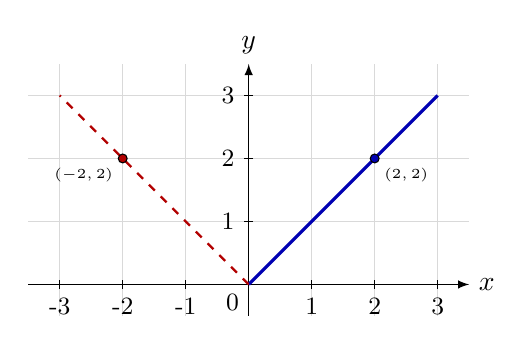
\begin{tikzpicture}[scale=0.8, >=latex]
    \draw[very thin, color=gray!30] (-3.5,-0.5) grid (3.5,3.5);
    \draw[->] (-3.5,0) -- (3.5,0) node[right] {$x$};
    \draw[->] (0,-0.5) -- (0,3.5) node[above] {$y$};
    
    \foreach \x in {-3,-2,-1,1,2,3}
        \draw (\x,2pt) -- (\x,-2pt) node[below, font=\small] {\x};
    \foreach \y in {1,2,3}
        \draw (2pt,\y) -- (-2pt,\y) node[left, font=\small] {\y};
    \node[below left, font=\small] at (0,0) {$0$};
    
    % Original part for [0, 3)
    \draw[very thick, color=blue!70!black] (0,0) -- (3,3);
    \filldraw[fill=blue!70!black] (2,2) circle (2pt) node[below right, font=\tiny] {$(2,2)$};
    
    % Symmetry reflection (Even)
    \draw[thick, dashed, color=red!70!black] (0,0) -- (-3,3);
    \filldraw[fill=red!70!black] (-2,2) circle (2pt) node[below left, font=\tiny] {$(-2,2)$};
\end{tikzpicture}
\end{center}

\monades{10}
\end{alist}
